\documentclass{article}

\usepackage{amsmath}
\usepackage{amssymb}
\usepackage{hyperref}
\usepackage{url}
\usepackage{graphicx}
\usepackage{geometry}
\usepackage{enumitem}
\usepackage{parskip}
\usepackage{chemfig}
\usepackage{pdfpages}
\usepackage{xcolor}
\usepackage{tikz}
\usepackage{fancybox}
\usepackage{makecell}
\usepackage{pgfplots}
\usepackage{soul}
\usepackage{ulem}
\usepackage{wrapfig}
\usepackage{subcaption}
\usepackage[T1]{fontenc}
\usepackage{esvect}
\usepackage{multirow}
\usepackage{booktabs}
\usepackage{float}
\usepackage{tocloft}
\usepackage{caption}
\usetikzlibrary{arrows}
\usetikzlibrary{decorations.pathreplacing}
\pgfplotsset{compat=1.17}
\usepgfplotslibrary{statistics}
\definecolor{darkgray}{rgb}{0.2, 0.2, 0.2}

% === BIBLIOGRAPHY ===
\usepackage[utf8]{inputenc}
\usepackage{csquotes}
\usepackage[style=apa, backend=biber, doi=true, url=true]{biblatex}
\addbibresource{ref.bib}
\DeclareFieldFormat[article]{volume}{\textbf{#1}}
\DeclareFieldFormat[article]{journaltitle}{\textit{#1}}
% ====================
 
\geometry{
    a4paper,
    total={170mm, 257mm},
    left=20mm,
    top=20mm
}

\hypersetup{
    colorlinks=true,
    linkcolor=black,
    urlcolor=blue,
    pdftitle={Report SW05 - EnCheBio}
}

\newcommand{\figbox}[1]{ 
    \begin{figure*}[ht!]        
        \begin{center}            
            \fbox{#1}        
        \end{center}    
    \end{figure*}
}

\newcommand{\wrapfill}{
    \par
    \ifnum \value{WF@wrappedlines} > 0
        \addtocounter{WF@wrappedlines}{-1}%
        \null\vspace{
            \arabic{WF@wrappedlines}
            \baselineskip
        }
        \WFclear
    \fi
    \phantom{}
}

\newcommand{\cfig}[1]{%
  \begin{figure*}[ht!]%
    \centering%
    #1%
  \end{figure*}%
}

% === LIST OF EQUATIONS ===
\newcounter{myequation}
\renewcommand{\themyequation}{\arabic{myequation}}

\newlistof{myequations}{loe}{\Large List of Equations}
\newcommand{\addequationtotoc}[1]{\addcontentsline{loe}{myequations}{\protect\numberline{\themyequation}#1}}

\renewcommand{\cftmyequationspresnum}{}
\renewcommand{\cftmyequationsaftersnum}{\hspace{1em}}
\setlength{\cftmyequationsnumwidth}{2em}
\cftsetindents{myequations}{1.5em}{2.3em}

\newcommand{\capeq}[3]{
    \refstepcounter{myequation}
    \begin{equation*}
        #1
    \end{equation*}
    \label{#2}
    \begin{center}
        \vspace*{-.4cm}
        \noindent{Equation \themyequation:} #3
    \end{center}
    \addequationtotoc{#3}
}

\newcommand{\refeq}[1]{\hyperref[#1]{[Equation~\ref*{#1}]}}
% =========================

\newcommand{\difference}{\,\backslash\,}
\newcommand{\rem}{\underline{Remark}: }
\newcommand{\nots}{\underline{Notation}: }
\newcommand{\prf}{\underline{Proof}: }
\newcommand{\exs}{\underline{Example}: }
\newcommand{\defs}{\underline{Definition}: }
\newcommand{\wrn}{\underline{Warning}: }
\newcommand{\sht}{\ |\ }
\newcommand{\pph}[1]{\paragraph{#1}\phantom{}\\}

% === TEXT ===
\title{\textbf{Practical 1 \\ Environmental chemistry and biology \\ HSLU, Semester 1}}
\author{Matteo Frongillo}

\begin{document}

\hypersetup{citecolor=black}

\begin{minipage}{0.7\textwidth}
    \vspace*{-.8cm} \hspace*{-0.3cm}
    
\includegraphics[width=.5\textwidth]{media/hslu-logo.png}
\end{minipage}

\vspace*{2cm}

\textbf{\huge Practical 1:}\\[.75cm]
\begin{center}
    \textbf{\huge Composting Parameters and}
    
    \textbf{\huge Plant Tolerance Test}\\[1cm]
    
    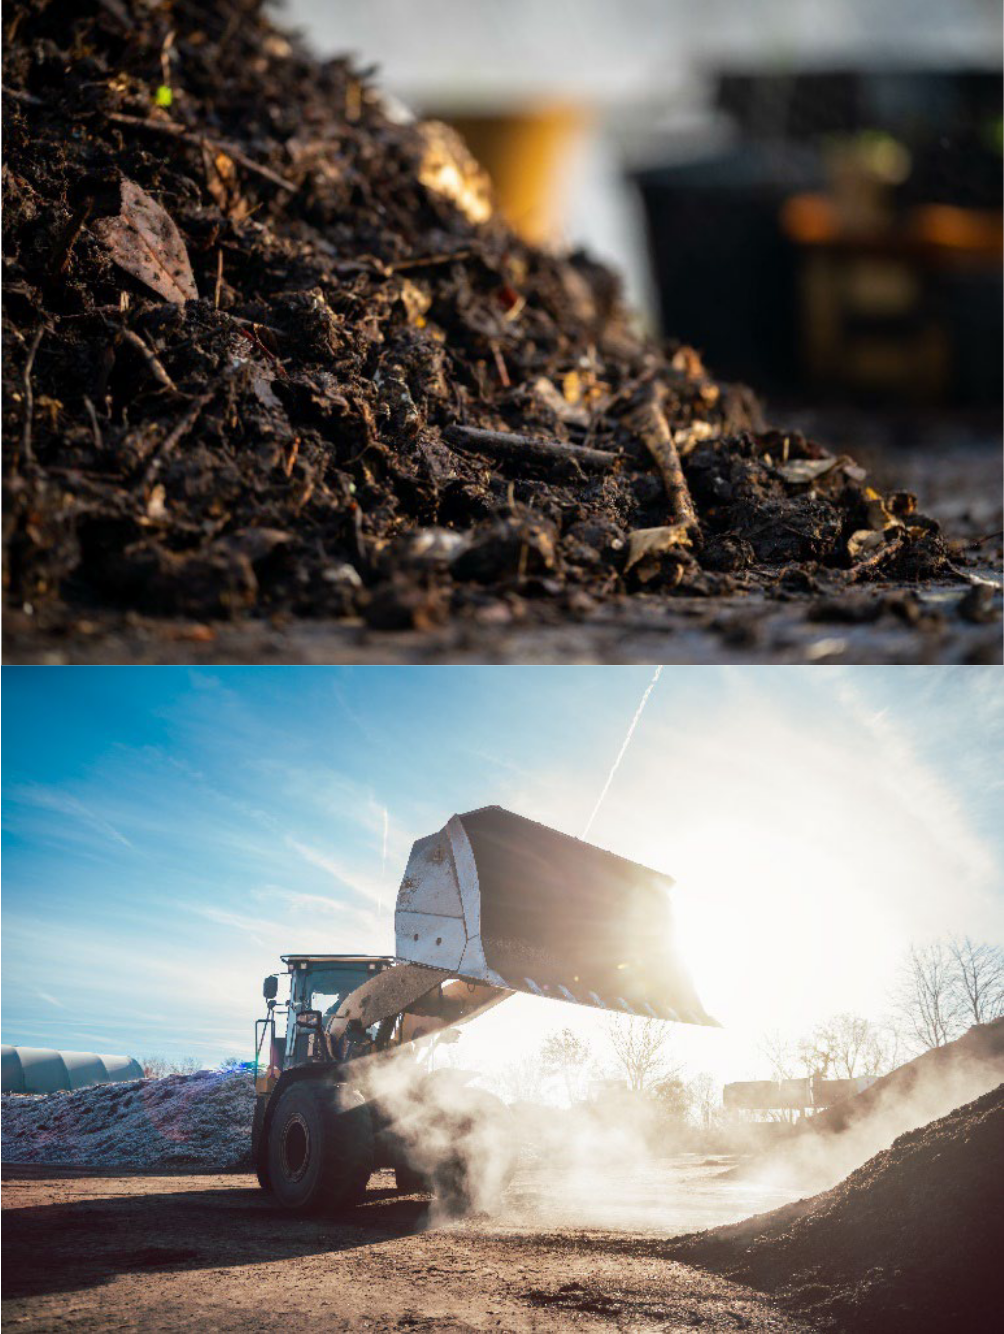
\includegraphics[width=0.6\textwidth]{media/front_practical1.png}\\
\end{center}

\vspace*{1cm}

\setlength{\intextsep}{0pt}%
\begin{wrapfigure}{r}{\textwidth}
    \textbf{\Large Environmental Chemistry and Biology HS2024\\[.5cm]
    \large Dr. Macarena San Martín Ruiz\\
    Lecturer}
    \vspace{-2.1cm}
\end{wrapfigure}

\phantom{}\\[-1cm]

\begin{flushright}
        \large
        \textbf{Team 4}\\
        Matteo Frongillo\\
        Ramadhan Nura\\
        Folagbade Popoola\\
        Jonathan Lawrence Boms\\
        Kron Xhemajli
\end{flushright}
\wrapfill

\tableofcontents
\pagebreak

\section{Introduction}
This experiment focuses on understanding how different types of compost affect plant
growth. It aims to explore the chemical and physical interactions between compost and
plant systems. Gaining a better understanding of these processes is essential for
improving sustainable farming methods, making nutrients more available to plants, and
managing resources effectively in agriculture.

\section{Materials and methods}
For this experiment, six gardening pots, three buckets containing different types of 
compost, a containment box, and a sieve were provided.

A scale and a measuring cylinder were used to determine the mass of the compost types
(fresh, standard, and finished). The initial and final temperatures at the bottom of each
pot were measured using a probe thermometer. Subsequently, pH measurements were conducted on each type of compost, with the samples
dissolved in distilled water in a small beaker. Next, the composts were placed into different pots and divided into three distinct
groups: 50\% finished and 25\% finished compost, 50\% fresh and 25\% fresh compost, and
standard soil.

Finally, 15 seeds were carefully placed in each pot, and their growth and development
were closely monitored.

\subsection{Pictures of proceedings}
\vspace*{.5cm}
\begin{figure}[ht!]
    \begin{minipage}[b]{0.5\textwidth}
        \centering
        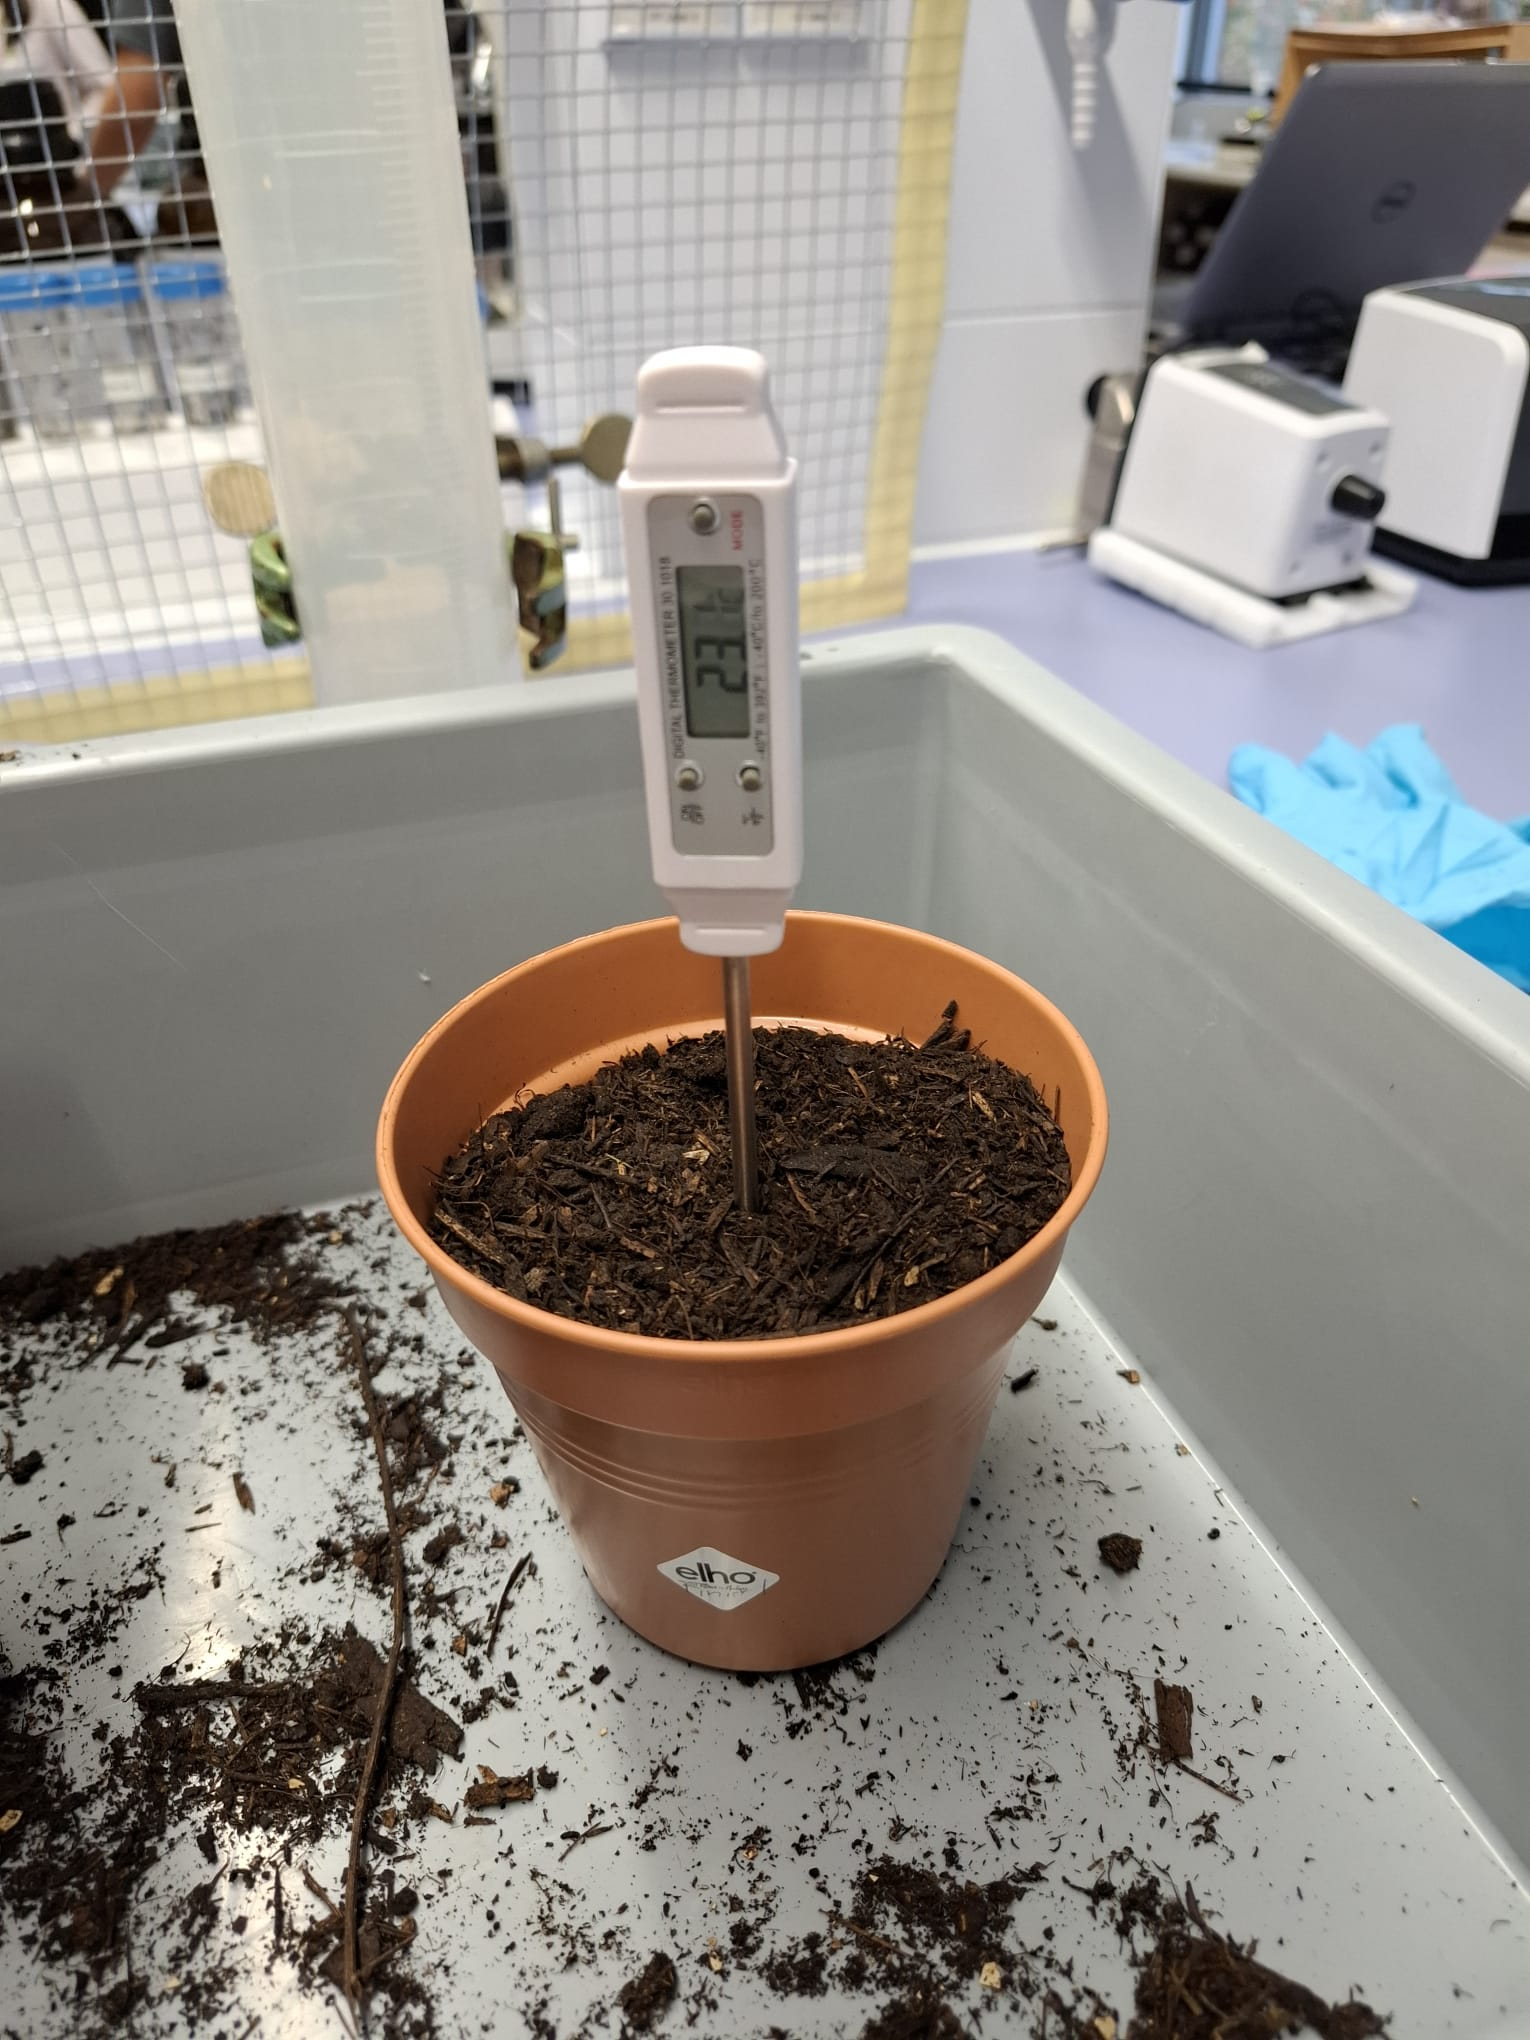
\includegraphics[width=.5\textwidth]{media/pot-temp.jpeg}
        \caption{Pot temperature}
    \end{minipage}%
    \hfill
    \begin{minipage}[b]{0.5\textwidth}
        \centering
        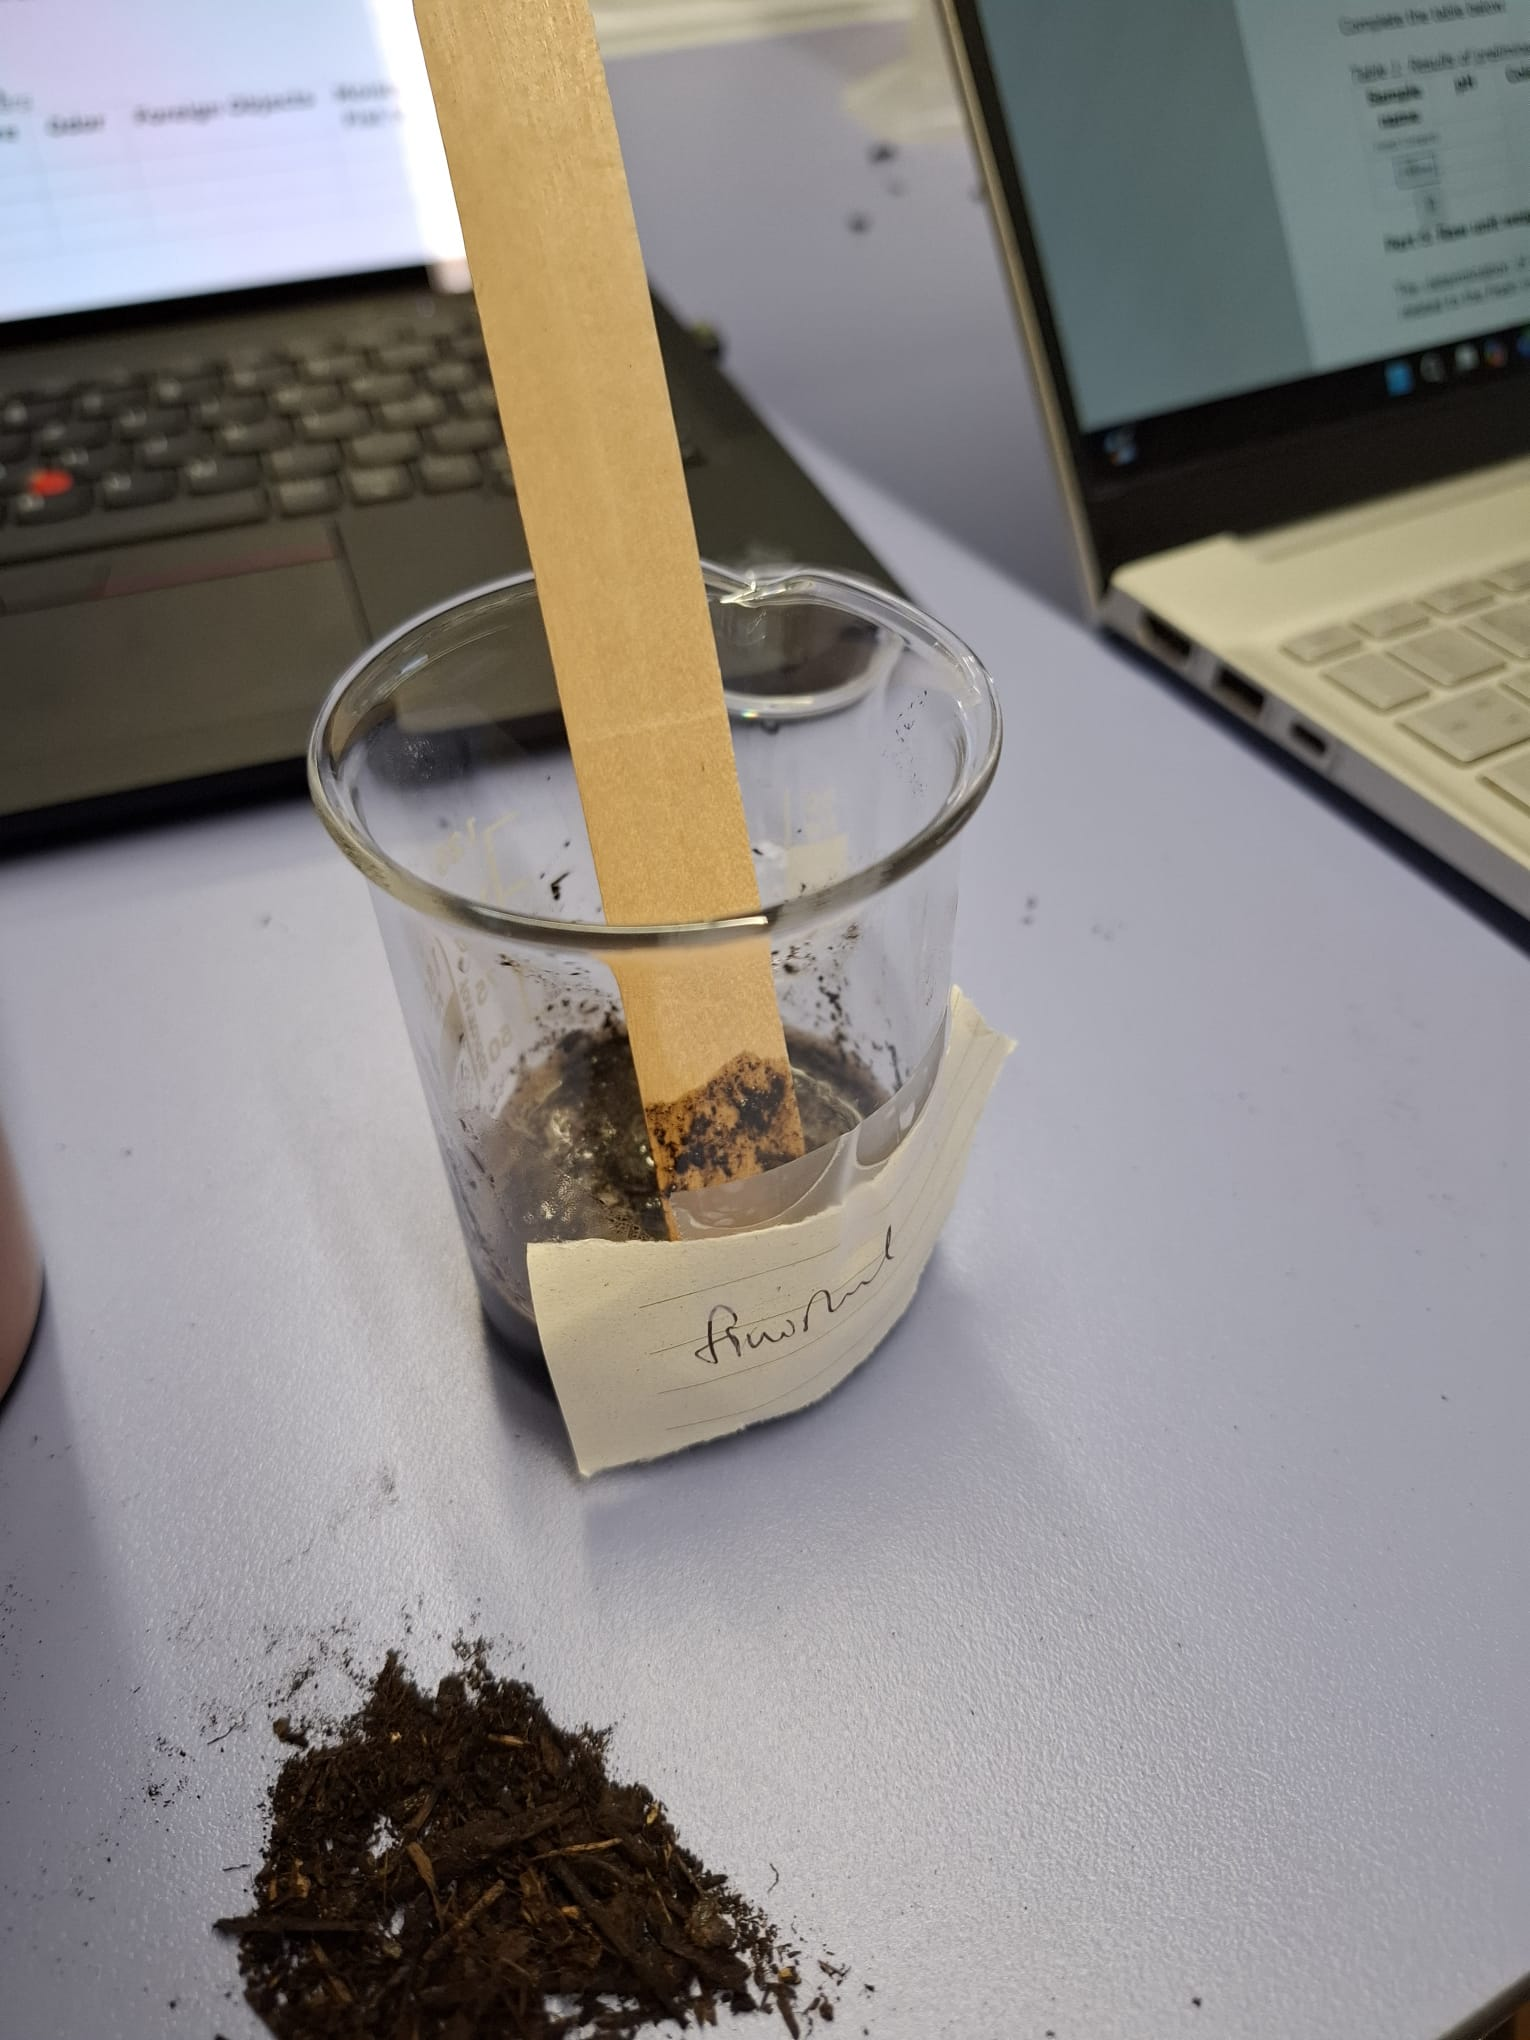
\includegraphics[width=.5\textwidth]{media/ph-mix.jpeg}
        \caption{Compost dissolution}
    \end{minipage}%
\end{figure}
\vspace*{1cm}

\begin{figure}[ht!]
    \begin{minipage}[b]{0.5\textwidth}
        \centering
        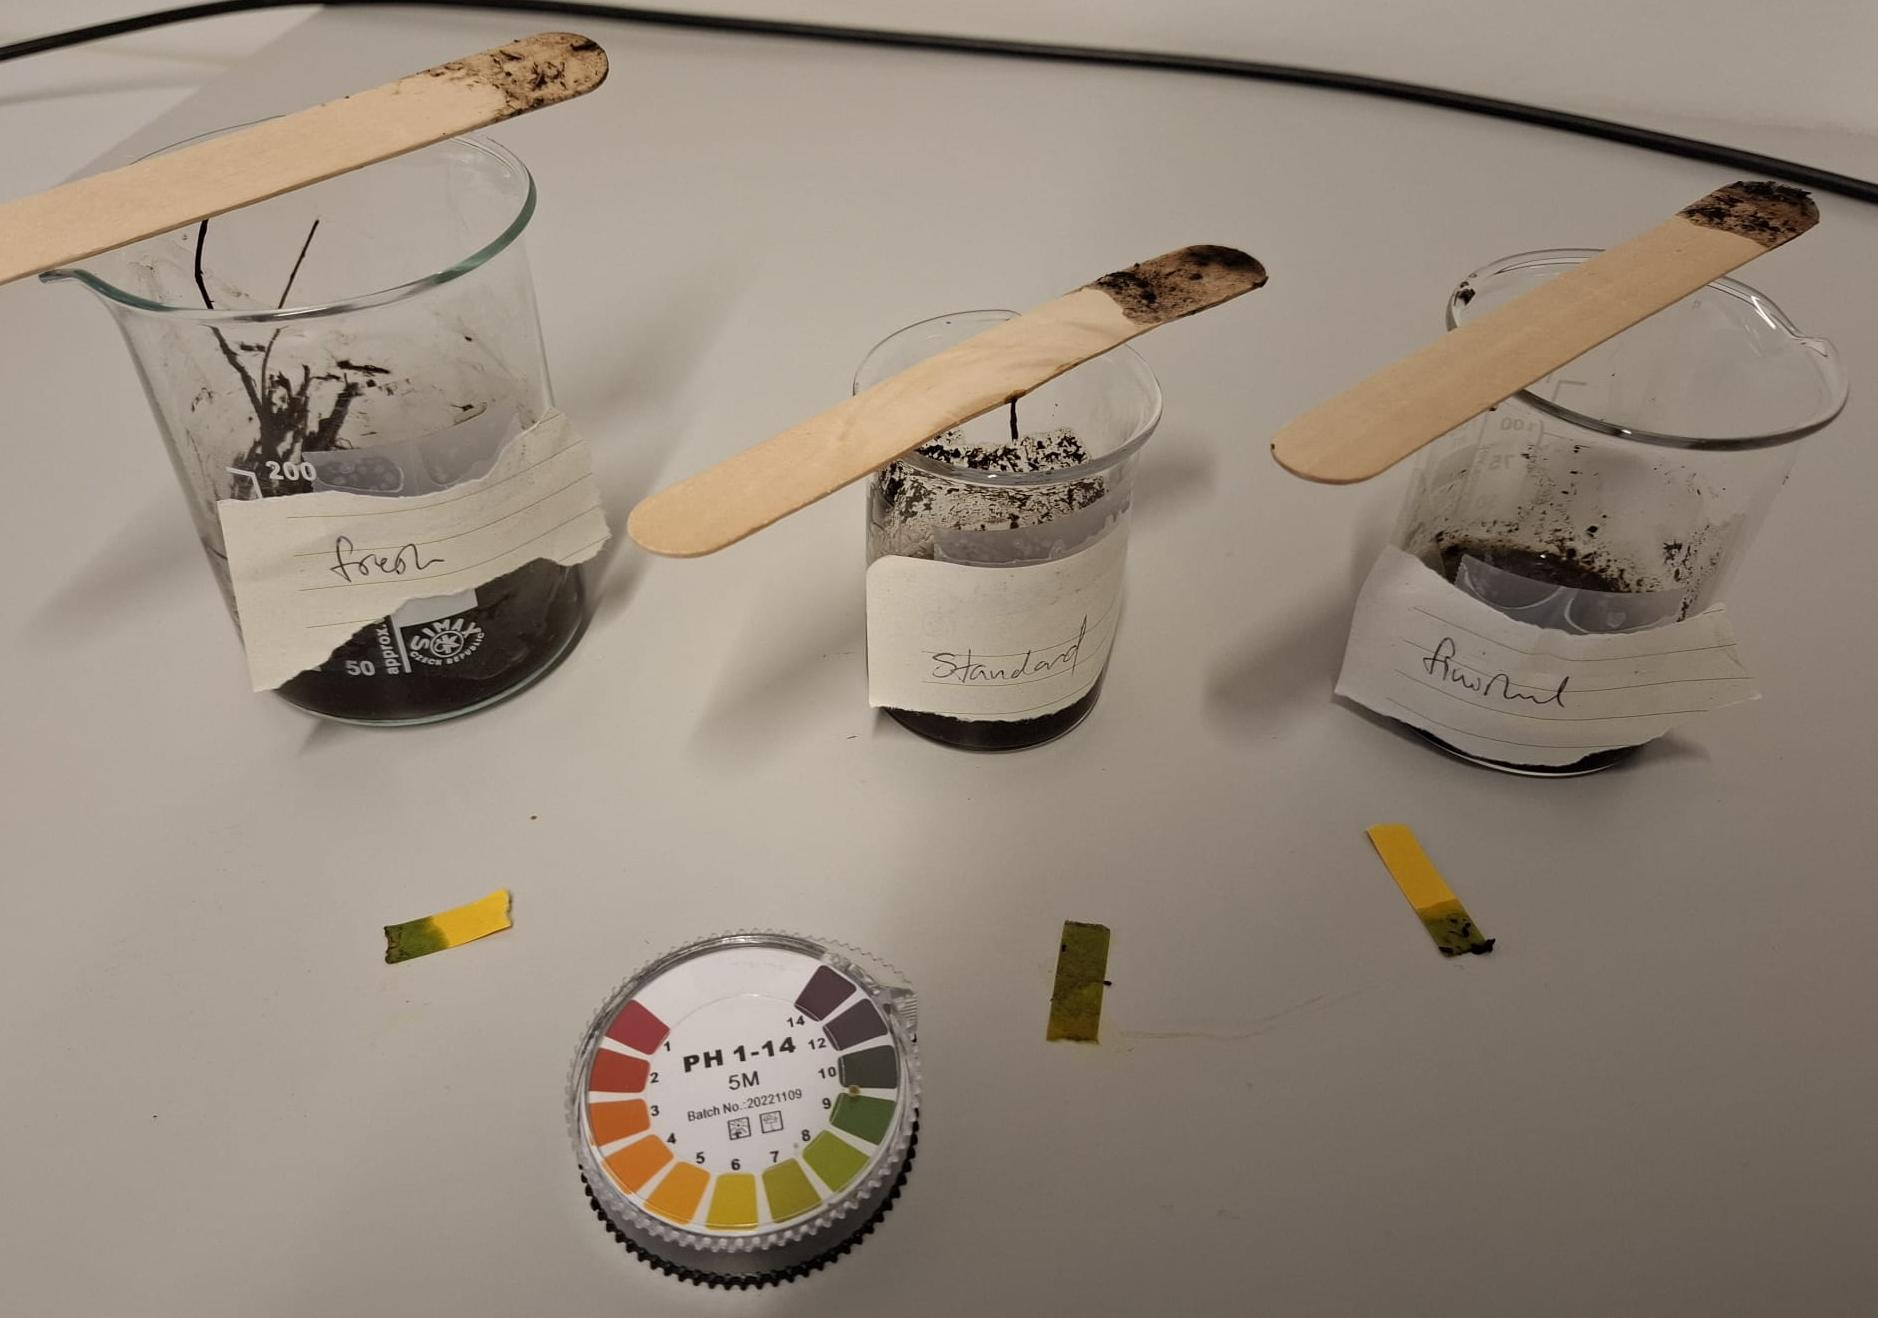
\includegraphics[width=\textwidth]{media/ph-results.jpeg}
        \caption{Compost pH results}
    \end{minipage}
    \hfill
    \begin{minipage}[b]{0.5\textwidth}
        \centering
        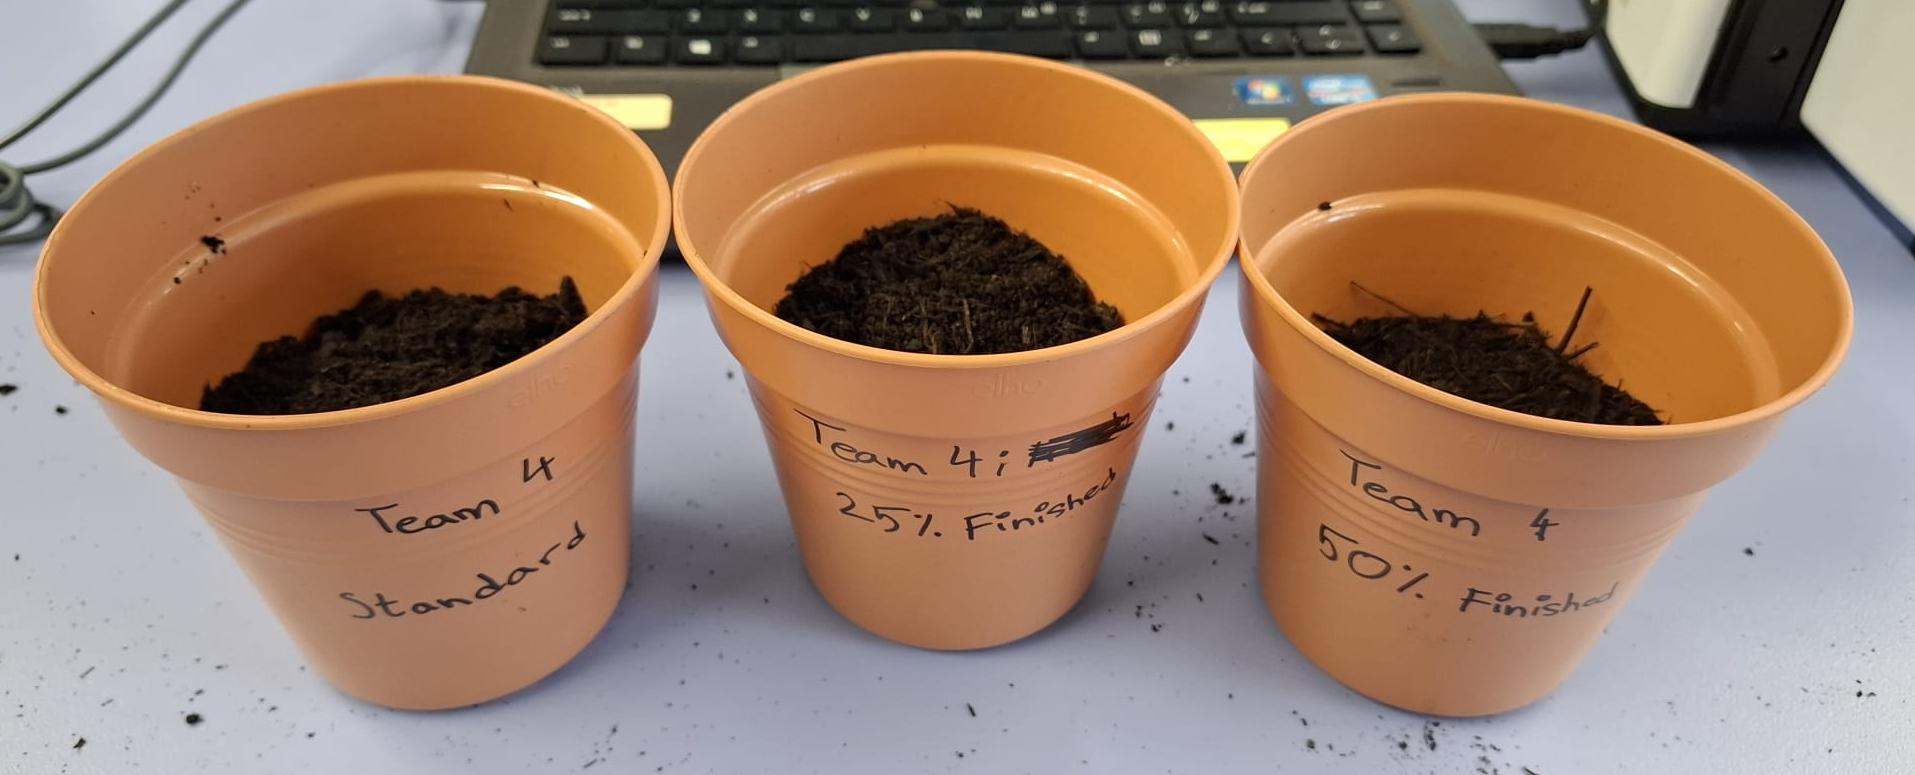
\includegraphics[width=\textwidth]{media/pots.jpeg}
        \caption{Triplet of compost inside the pots}
    \end{minipage}
\end{figure}
\vspace*{.5cm}

\newpage
\section{Results}
\subsection{Preliminary parameters}
We collected three samples: Fresh, Finished, and Standard, and 
valuated them based on several characteristics, including pH, color,
texture, odor, foreign objects, and moisture content. Each sample had
distinct features, which helped us assess their condition and quality. 

\subsubsection{Preliminary parameters table}
\renewcommand{\arraystretch}{1.5}
\begin{table*}[ht!]
    \centering \vspace{.3cm}
    \caption{Results of preliminary parameters}
    \hspace*{-.3cm}
    \begin{tabular}{|c|c|c|c|c|c|c|}
        \hline
        \textbf{Sample} & \textbf{pH} & \textbf{Color} & \textbf{Texture} & \textbf{Odor} & \textbf{Foreign objects} & \textbf{Moisture fist test}\\
        \hline
        \multirow{2}{*}{Fresh} & \multirow{2}{*}{9} & \multirow{2}{*}{Light brown} & \multirow{2}{*}{Coarse} & \multirow{2}{*}{Smells ammonia} & Large roots & \multirow{2}{*}{30\% humidity} \\
        & & & & & and plastics & \\
        \hline                                                                  
        \multirow{2}{*}{Finished} & \multirow{2}{*}{8} & \multirow{2}{*}{Dark brown} & \multirow{2}{*}{Fine} & \multirow{2}{*}{Smells ammonia} & Sticks and & \multirow{2}{*}{20\% humidity} \\
        & & & & & plastic particles & \\
        \hline
        Standard & 7 & Darkest brown & Clumpy & Smells earthy & -- & 30\% humidity\\
        \hline
    \end{tabular}
\end{table*}
\phantom{} \vspace*{-.2cm}

\subsubsection{Compost temperature}
The temperature of different composts was measured so that an
assessment could be made of how favorable germination was within the
compost. For the measurements, the probe thermometer was allowed to
rest inside the compost for 5 minutes, and the initial and final
temperatures were recorded.

\begin{table*}[ht!]
    \centering \vspace{.3cm}
    \caption{Compost temperature}
    \hspace*{-.3cm}
    \begin{tabular}{|c|c|c|c|}
        \hline
        \textbf{Sample} & \textbf{Initial} [$^\circ$C] & \textbf{Final} [$^\circ$C] & \textbf{Mean temp.} [$^\circ$C]\\
        \hline
        Fresh & 23.8 & 23.7 & 23.75 \\
        \hline
        Finished & 23.2 & 23.0 & 23.1\\
        \hline
        Standard & \multicolumn{3}{c|}{23.5}\\
        \hline
    \end{tabular}
\end{table*}

\vspace*{.5cm}
\subsection{Fresh, Finished and Standard compost}
Three samples were collected, and their raw unit weight was evaluated.
The mass of the empty cylinder was measured in grams, with a value of
168.24 g. The mass of the filled cylinder for each sample was then
measured, obtaining values in liters. The volume of each sample was
also measured in milliliters. Using these measurements, the density
results were calculated in both [kg/L] and [kg/m$^3$] using the formulas:

\capeq{\text{Density} \left[kg/L\right] = \frac{\text{Mass of filled cylinder}\ [g] - \text{Mass of empty cylinder}\ [g]}{\text{Volume of sample}\ [mL]}}{eq:density1}{Density formula in $[kg/L]$}

\capeq{\text{Density} \left[kg/m^3\right] = \text{Density} \left[kg/L\right] \cdot 1000 \left[L/m^3\right]}{eq:density2}{Density formula in $[kg/m^3]$}

The average values provided insight into the consistency of the raw
unit weight across the different samples.

\newpage
\subsubsection{Fresh compost}
\renewcommand{\arraystretch}{1.5}
\begin{table*}[ht!]
    \centering \vspace{.3cm}
    \caption{Results of raw unit weight in three different samples of fresh compost}
    \begin{tabular}{|c|c|c|c|c|}
        \hline
        \textbf{Sample} & \textbf{1} & \textbf{2} & \textbf{3} & \textbf{Average}\\
        \hline
        {\textbf{Mass of the empty}} & \multicolumn{4}{c|}{\multirow{2}{*}{168.24}}\\
        \textbf{cylinder in [g]} & \multicolumn{4}{c|}{}\\
        \hline
        \textbf{Mass of the filled} & \multirow{2}{*}{120.88} & \multirow{2}{*}{112.20} & \multirow{2}{*}{108.71} & \multirow{2}{*}{113.93}\\
        \textbf{cylinder [g]} & & & &\\
        \hline
        \textbf{Volume of the} & \multirow{2}{*}{340} & \multirow{2}{*}{330} & \multirow{2}{*}{390} & \multirow{2}{*}{353.33}\\
        \textbf{sample in [mL]} & & & &\\
        \hline
        \textbf{Result in [kg/L]} & 0.356 & 0.34 & 0.279 & 0.325\\
        \hline
        \textbf{Result in [kg/m$^3$]} & 356 & 340 & 279 & 325\\
        \hline
    \end{tabular}
\end{table*}

\subsubsection{Finished compost}
\renewcommand{\arraystretch}{1.5}
\begin{table*}[ht!]
    \centering \vspace{.3cm}
    \caption{Results of raw unit weight in three different samples of finished compost}
    \begin{tabular}{|c|c|c|c|c|}
        \hline
        \textbf{Sample} & \textbf{1} & \textbf{2} & \textbf{3} & \textbf{Average}\\
        \hline
        {\textbf{Mass of the empty}} & \multicolumn{4}{c|}{\multirow{2}{*}{168.24}}\\
        \textbf{cylinder in [g]} & \multicolumn{4}{c|}{}\\
        \hline
        \textbf{Mass of the filled} & \multirow{2}{*}{214.54} & \multirow{2}{*}{202.91} & \multirow{2}{*}{202.68} & \multirow{2}{*}{206.71}\\
        \textbf{cylinder [g]} & & & &\\
        \hline
        \textbf{Volume of the} & \multirow{2}{*}{375} & \multirow{2}{*}{370} & \multirow{2}{*}{380} & \multirow{2}{*}{375}\\
        \textbf{sample in [mL]} & & & &\\
        \hline
        \textbf{Result in [kg/L]} & 0.572 & 0.548 & 0.533 & 0.551\\
        \hline
        \textbf{Result in [kg/m$^3$]} & 572 & 548 & 533 & 551\\
        \hline
    \end{tabular}
\end{table*}

\subsubsection{Standard compost}
\renewcommand{\arraystretch}{1.5}
\begin{table*}[ht!]
    \centering \vspace{.3cm}
    \caption{Results of raw unit weight in three different samples of standard compost}
    \begin{tabular}{|c|c|c|c|c|}
        \hline
        \textbf{Sample} & \textbf{1} & \textbf{2} & \textbf{3} & \textbf{Average}\\
        \hline
        {\textbf{Mass of the empty}} & \multicolumn{4}{c|}{\multirow{2}{*}{168.24}}\\
        \textbf{cylinder in [g]} & \multicolumn{4}{c|}{}\\
        \hline
        \textbf{Mass of the filled} & \multirow{2}{*}{222.95} & \multirow{2}{*}{228.44} & \multirow{2}{*}{212.74} & \multirow{2}{*}{221.38}\\
        \textbf{cylinder [g]} & & & &\\
        \hline
        \textbf{Volume of the} & \multirow{2}{*}{355} & \multirow{2}{*}{370} & \multirow{2}{*}{360} & \multirow{2}{*}{361.67}\\
        \textbf{sample in [mL]} & & & &\\
        \hline
        \textbf{Result in [kg/L]} & 0.628 & 0.617 & 0.591 & 0.612\\
        \hline
        \textbf{Result in [kg/m$^3$]} & 628 & 617 & 591 & 612\\
        \hline
    \end{tabular}
\end{table*}

\newpage
\subsection{Experiment results}
\renewcommand{\arraystretch}{1.5}
\begin{table*}[ht!]
    \centering \vspace{.3cm}
    \caption{Experiment results}
    \begin{tabular}{|l|c|c|c|c|c|c|}
        \hline
        \textbf{Group 4} & \textbf{E0} & \textbf{E0} & \textbf{E25} & \textbf{E25} & \textbf{E50} & \textbf{E50} \\
        \hline
        mean compost density (kg/L) & \multicolumn{2}{c|}{0.325} & \multicolumn{2}{c|}{0.382} & \multicolumn{2}{c|}{0.438}\\
        \hline
        n$^{\circ}$ germinated seeds & 12 & 13 & 11 & 12 & 11 & 10\\
        \hline
        plants weight (g) & 1.672 & 1.882 & 0.997 & 1.294 & 1.058 & 1.105\\
        \hline
    \end{tabular}
\end{table*}

\vspace*{.7cm}
\begin{figure}[ht!]
    \centering
    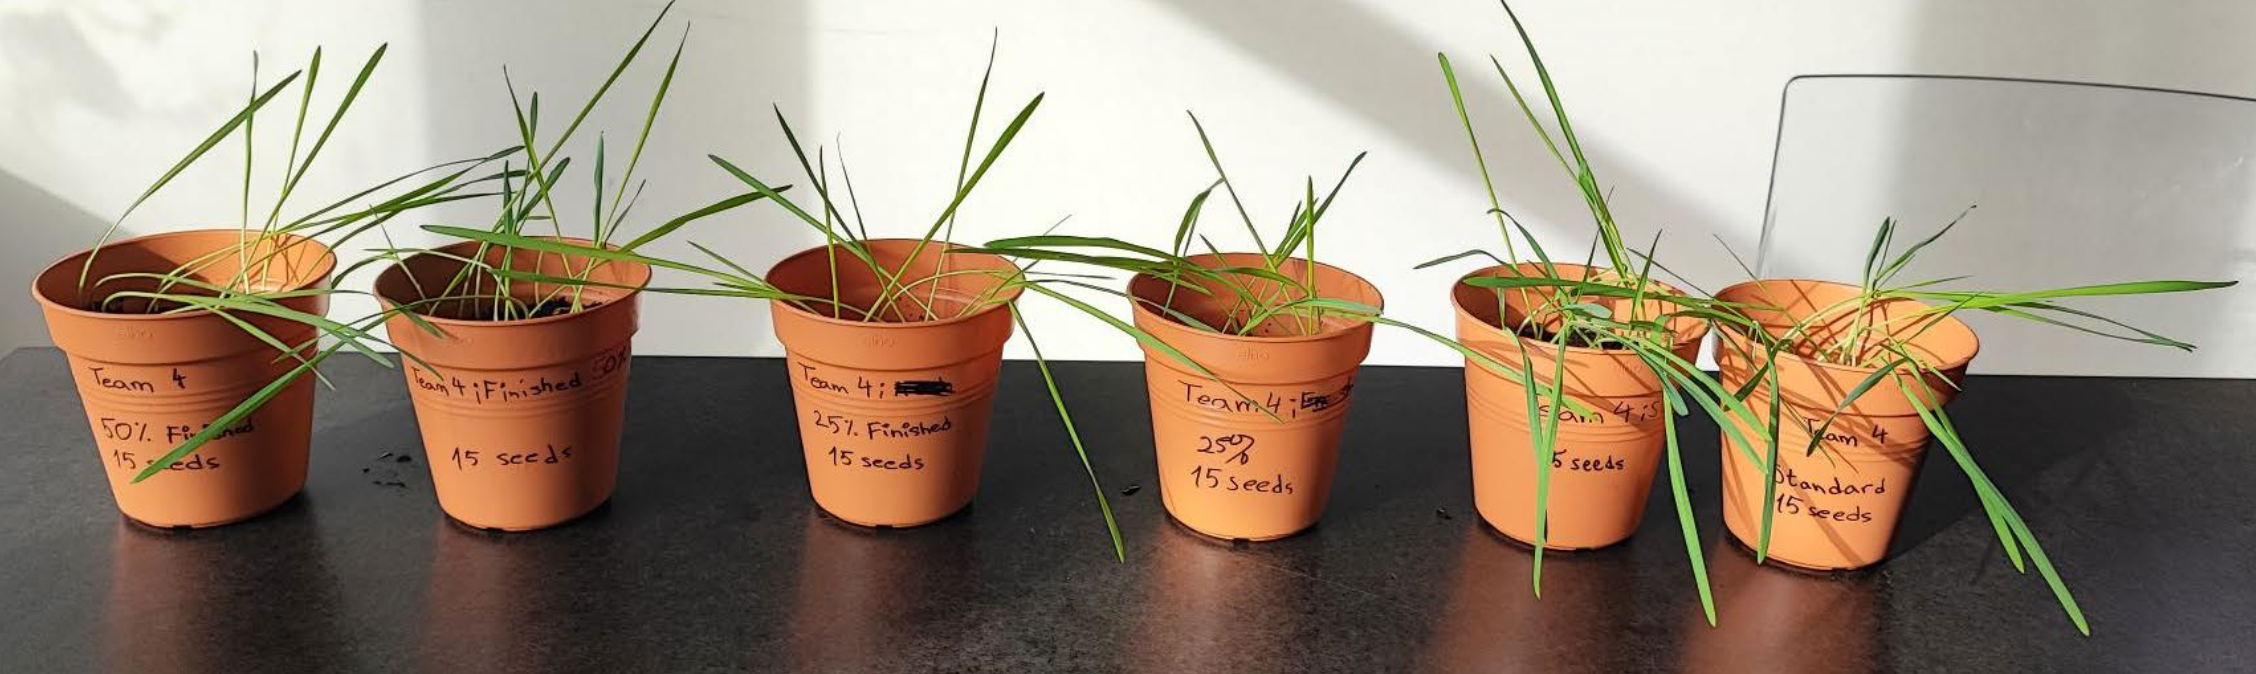
\includegraphics[width=.9\textwidth]{media/plants-results.png}
    \caption{Growth status 2 weeks after insemination}
\end{figure}

\vspace*{.5cm}
From the comparison of the different treatments, it is observed that compost E0 promoted
both germination and plant growth in terms of biomass, with superior results compared to
E25 and E50. The figure clearly shows that the plants treated with E0 are more developed
compared to the other treatments. Treatments E25 and E50, with increasing percentages of
finished compost, show limited growth.

\subsection{Statistical formulas}
For statistical analysis, the formulas mentioned below are used:
\begin{itemize}
    \item \textbf{Arithmetic mean} ($\overline{x}$):
    \capeq{\overline{x} = \frac{1}{n} \sum_{i=1}^{n} x_i}{eq:mean}{Arithmetic mean formula}

    \underline{Please note}: since the class consists of two data points,
        the \textbf{median} corresponds to the arithmetic mean. 
    \item \textbf{Variance} ($\sigma^2$):
    \capeq{\sigma^2 = \frac{1}{n-1} \sum_{i=1}^{n} (x_i - \overline{x})^2}{eq:variance}{Variance formula}
    \item \textbf{Standard deviation} ($\sigma$):
    \capeq{\sigma = \sqrt{\sigma^2}}{eq:stdev}{Standard deviation formula}
\end{itemize}

\newpage
\subsection{Statistical analysis for germinated seeds}
\subsubsection{Analysis for E0}
\pph{Data set}
The E0 group class consists of the data [12,13] for the number of sprouted seeds,
respectively [1.672g, 1.882g] for their mass.

\pph{Arithmetic mean and median}
\capeq{\overline{x}_{E0} = \frac{12+13}{2} = 12.5}{eq:e0_mean}{Arithmetic mean and median of germinated E0}

\capeq{\overline{m}_{E0} = \frac{1.672g + 1.882g}{2} = 1.78g}{eq:e0_mass}{Arithmetic mean and median of E0 plants mass}

\pph{Variance and standard deviation}
\capeq{\sigma_{x,E0} = \sqrt{\frac{(12-12.5)^2 + (13-12.5)^2}{2-1}} = \sqrt{0.5} \approx 0.707}{eq:e0_dev}{Standard deviation of germinated E0}

\capeq{\sigma_{m,E0} = \sqrt{\frac{(1.672g - 1.777g)^2 + (1.882g - 1.777g)^2}{2-1}} \approx 0.148g}{eq:e0_mass_dev}{Standard deviation of E0 plants mass}

\subsubsection{Analysis for E25}
\pph{Data set}
The E25 group class consists of the data [11,12] for the number of sprouted seeds,
respectively [0.997g, 1.294g] for their mass.

\pph{Arithmetic mean and median}
\capeq{\overline{x}_{E25} = \frac{11+12}{2} = 11.5}{eq:e25_mean}{Arithmetic mean and median of E25}

\capeq{\overline{m}_{E25} = \frac{0.997g + 1.294g}{2} = 1.15g}{eq:e25_mass}{Arithmetic mean and median of E25 plants mass}

\pph{Variance and standard deviation}
\capeq{\sigma_{x,E25} = \sqrt{\frac{(11-11.5)^2 + (12-11.5)^2}{2-1}} = \sqrt{0.5} \approx 0.707}{eq:e25_dev}{Standard deviation of E25}

\capeq{\sigma_{m,E25} = \sqrt{\frac{(0.997g-1.146g)^2 + (1.294g-1.146g)^2}{2-1}} \approx 0.210g}{eq:e25_mass_dev}{Standard deviation of E25 plants mass}

\subsubsection{Analysis for E50}
\pph{Data set}
The E50 group class consists of the data [10,11] for the number of sprouted seeds,
respectively [1.058g, 1.105g] for their mass.

\pph{Arithmetic mean and median}
\capeq{\overline{x}_{E50} = \frac{10+11}{2} = 10.5}{eq:e50_mean}{Arithmetic mean and median of E50}

\capeq{\overline{m}_{E50} = \frac{1.058g + 1.105g}{2} = 1.08g}{eq:e50_mass}{Arithmetic mean and median of E50 plants mass}

\pph{Variance and standard deviation}
\capeq{\sigma_{x,E50} = \sqrt{\frac{(10-10.5)^2 + (11-10.5)^2}{2-1}} = \sqrt{0.5} \approx 0.707}{eq:e50_dev}{Standard deviation of E50}

\capeq{\sigma_{m,E50} = \sqrt{\frac{(1.058g-1.082g)^2 + (1.105g-1.082g)^2}{2-1}} \approx 0.0333g}{eq:e25_mass_dev}{Standard deviation of E50 plants mass}

\subsubsection{Summary table}
\renewcommand{\arraystretch}{1.5}
\begin{table*}[ht!]
    \centering \vspace{.3cm}
    \caption{Statistical analysis by number of germinated seeds}
    \begin{tabular}{|c|c|c|c|c|}
        \hline
        & E0 & E25 & E50 & Overall mean\\
        \hline
        \textbf{mean and mediane} & 12.5 & 11.5 & 10.5 & 11.5\\
        \hline
        \textbf{standard deviation} & \multicolumn{4}{c|}{0.707}\\
        \hline
    \end{tabular}
\end{table*}

\vspace*{1cm}
\renewcommand{\arraystretch}{1.5}
\begin{table*}[ht!]
    \centering \vspace{.3cm}
    \caption{Statistical analysis for the weight of germinated seeds}
    \begin{tabular}{|c|c|c|c|c|}
        \hline
        & E0 & E25 & E50 & Overall mean\\
        \hline
        \textbf{mean and median} [g] & 1.78 & 1.15 & 1.08 & 1.34\\
        \hline
        \textbf{standard deviation} [g] & 0.148 & 0.210 & 0.0333 & 0.131\\
        \hline
    \end{tabular}
\end{table*}
\vspace*{.5cm}

\newpage
\subsection{Relative yield}
To calculate the relative yield $FM(r)$ at 25\% and 50\% using the data from the table,
we can use this formula:

\capeq{FM(r) \% = \frac{FM \%}{E0\%} \cdot 100}{eq:yield}{Relative yield $FM(r)$}

\subsubsection{Average $FM_{E0}$}
To calculate the average, the arithmetic mean formula was used \refeq{eq:mean}:

\capeq{FM_{E0} = \frac{1.672g + 1.882g}{2} = \frac{3.554g}{2} = 1.777g}{eq:fm_e0}{Average $FM_{E0}$}

\subsubsection{Calculation of the relative yields}
\begin{enumerate}
    \item \textbf{E25}:
        \capeq{FM(r)\ 25\% = \frac{0.997}{1.777} \cdot 100 = 56.1\%}{eq:first-e25}{Yield of the first E25\% pot}

        \capeq{FM(r)\ 25\% = \frac{1.294}{1.777} \cdot 100 = 72.8\%}{eq:second-e25}{Yield of the second E25\% pot}
  
    \item \textbf{E50}:
        \capeq{FM_1(r)\ 50\% = \frac{1.058}{1.777} \cdot 100 = 59.5\%}{eq:first-e50}{Yield of the first E50\% pot}

        \capeq{FM_2(r)\ 50\% = \frac{1.105}{1.777} \cdot 100 = 62.2\%}{eq:second-e50}{Yield of the second E50\% pot}
\end{enumerate}

\subsubsection{Summary table}
\renewcommand{\arraystretch}{1.5}
\begin{table*}[ht!]
    \centering \vspace{.3cm}
    \caption{Relative yields}
    \begin{tabular}{|c|c|c|c|}
        \hline
        & E25 & E50 & Overall mean\\
        \hline
        \textbf{FM(r) 25\%} & 56.1\% & 72.8\% & 64.5\%\\
        \hline
        \textbf{FM(r) 50\%} & 59.5\% & 62.2\% & 60.9\%\\
        \hline
    \end{tabular}
\end{table*}
\vspace*{.5cm}

The FM (r) results indicate that E25 compost has a relative yield of
64.5 percent compared to E0 reference compost, while E50 compost has
a relative yield of 60.9 percent. These values indicate that composts
with higher percentages of finished compost have a lower yield than
standard compost, showing what even a small fraction of an average
finished compost causes to the plants.

\subsection{Graphical results}
Data visualized through boxplots allow observing the distribution of
data obtained from the experiment and evaluating the performance of
different composts. The medians, quartiles and extremes of the data
allow visualizing the effectiveness of each type of compost with
respect to plant development.

\newpage
\subsubsection{Boxplot of germinated seeds}

\vspace*{.5cm}

\begin{figure}[h!]
    \centering
    \begin{tikzpicture}
        \begin{axis}[
            width=.8\textwidth,
            height=0.5\textwidth,
            boxplot/draw direction=y,
            ylabel={Number of germinated seeds},
            xlabel={Type of sample},
            xtick={1, 2, 3, 4},
            xticklabels={E0, E25, E50, Mean},
        ]
            \addplot+[
                boxplot prepared={
                    median=12.5,
                    upper quartile=13,
                    lower quartile=12,
                    upper whisker=13,
                    lower whisker=12
                },
            ] coordinates {};
            
            \addplot+[
                boxplot prepared={
                    median=11.5,
                    upper quartile=12,
                    lower quartile=11,
                    upper whisker=12,
                    lower whisker=11
                },
            ] coordinates {};
            
            \addplot+[
                boxplot prepared={
                    median=10.5,
                    upper quartile=11,
                    lower quartile=10,
                    upper whisker=11,
                    lower whisker=10
                },
            ] coordinates {};
            
            \addplot+[
                boxplot prepared={
                    median=11.5,
                    upper quartile=12.5,
                    lower quartile=10.5,
                    upper whisker=13,
                    lower whisker=10
                },
            ] coordinates {};
        \end{axis}
    \end{tikzpicture}
    \caption{Boxplot of the germination of different composts}
    \label{fig:boxplot_germinated}
\end{figure}

\vspace*{.5cm}
The boxplot shows the number of germinated seeds for the different
compost treatments: E0, E25, E50, and the ``mean'' group. It
can be observed that the E0 treatment has the highest median, and the E50
treatment has a lower median compared to the others, indicating a
decrease in effectiveness for seed germination as compost maturity
increases. The ``mean'' group displays the largest variability,
highlighting significant differences between the compost treatments
in terms of their ability to promote germination.

\subsubsection{Boxplot of plant mass}
\vspace*{.5cm}

\begin{figure}[h!]
    \centering
    \begin{tikzpicture}
        \begin{axis}[
            width=.8\textwidth,
            height=0.5\textwidth,
            boxplot/draw direction=y,
            ylabel={Plant mass [g]},
            xlabel={Type of sample},
            xtick={1, 2, 3, 4},
            xticklabels={E0, E25, E50, Mean},
        ]
            \addplot+[
                boxplot prepared={
                    median=1.78,
                    upper quartile=1.882,
                    lower quartile=1.672,
                    upper whisker=1.882,
                    lower whisker=1.672
                },
            ] coordinates {};
            
            \addplot+[
                boxplot prepared={
                    median=1.15,
                    upper quartile=1.294,
                    lower quartile=0.997,
                    upper whisker=1.294,
                    lower whisker=0.997
                },
            ] coordinates {};
            
            \addplot+[
                boxplot prepared={
                    median=1.08,
                    upper quartile=1.105,
                    lower quartile=1.058,
                    upper whisker=1.105,
                    lower whisker=1.058
                },
            ] coordinates {};
            
            \addplot+[
                boxplot prepared={
                    median=1.34,
                    upper quartile=1.78,
                    lower quartile=1.08,
                    upper whisker=1.882,
                    lower whisker=0.997
                },
            ] coordinates {};
        \end{axis}
    \end{tikzpicture}
    \caption{Boxplot of plant mass based on compost used}
    \label{fig:boxplot_mass}
\end{figure}

\vspace*{.5cm}
The boxplot shows the plant mass for different compost treatments:
E0, E25, E50, and the overall group. It can be observed that the E0
treatment yields the highest median plant mass, suggesting that this
compost type is the most effective in promoting plant growth. The E50
treatment has the lowest median, indicating reduced effectiveness in
supporting plant growth with increasing compost maturity. The ``mean''
group displays the largest variability, highlighting significant
differences between treatments.

\newpage
\section{Discussion}
\subsection{Results discussion}
\subsubsection{Compost}
The different compost combinations (E0, E25, E50) significantly influenced plant
germination. E0 provided the best conditions, likely due to an ideal nutrient balance and
physical properties. E25 and E50 showed reduced germination, possibly due to greater
chemical stability and less immediate nutrient availability.

\subsubsection{Influence of pH and Nitrogen cycle}
pH was an important factor in compost effectiveness. E0 had a balanced pH, favoring
microbial growth and seed germination. In contrast, E25 and E50 may have had less suitable
pH levels, affecting microbial activity and slowing nitrogen mineralization, reducing
germination effectiveness.

Finished compost in E25 and E50 may have increased denitrification, reducing available
nitrogen. Combined with reduced microbial activity, this limited nutrient availability in
early growth stages. E0 showed better biomass growth, indicating the importance of
immediate nutrient availability.

\subsubsection{Plants mass}
E0 was the most effective for plant growth by weight, providing readily available
nutrients. E50 showed reduced growth, suggesting that a higher proportion of finished
compost limited nutrient availability needed for early plant development.

\subsection{Questions}
\begin{enumerate}
    \item What is the difference between raw unit weight and bulk density? Discuss your
        results based on the laboratory experiment.

        \textbf{R:\\}
        Raw unit weight is the density given by the division of the mass of the compost
        over the volume of the compost. The bulk unit is the density given by the division
        of the mass of the compost over the volume of the container.

    \item How can the pH affect the compost?
    
        \textbf{R:\\}
        The more acidic the soil is, the more inactive the bacteria are, and this bring
        plants to not grow properly. Vice versa for the basicity.\\
        Compost microorganisms operate best under neutral to acidic conditions, with pH's
        in the range of 5.5 to 8. During the initial stages of decomposition, organic
        acids are formed. The acidic conditions are favourable for growth of fungi and
        breakdown of lignin and cellulose \parencite{cornell}.

    \item What is the impact of immature compost on plant growth, and how can this be
        assessed in the lab?

        \textbf{R:\\}
        Plants will not grow properly if the nitrogen cycle is not working. Indeed, it is
        generally accepted that compost produced with substrates rich in nitrogen will
        have a better fertilizing effect, compared to other compost whose substrates are
        mainly woody. Likewise, immature compost will have a repressive effect on seed
        germination and plant growth \parencite{tamakloe2021}.\\
        In the lab, we can do the germination test and for immature compost you have
        standard growth.

    \item How do you calculate the bulk density of compost, and why is this measurement
        important in the composting process?

        \textbf{R:\\}
        Divide the mass of the compost by the volume of the container. Bulk density
        provides an overall indication for the physical and aeration conditions of a
        composting mass \parencite{bulk_density}.

    \item What would be the environmental impact if fresh compost is added in the
        plantations/agriculture or when the recommended percentage of compost mixture
        is not followed?

        \textbf{R:\\}
        The addition of fresh compost may lead to suboptimal plant growth due to high
        biological activity and temperature, which could create unfavorable conditions for
        germination, compromising growth and plants and reduced yields. Deviation from the
        recommended compost mixture could result in inconsistent results that would lead to
        reduced germination and growth compared to standard compost \parencite{mladenov2018}.

\end{enumerate}

\subsection{Conclusion}
In this experiment, the effects of different types of compost (fresh, finished, and standard)
on seed germination over a one-week period were investigated. The results indicated that
fresh compost led to suboptimal seed growth due to its high biological activity and
temperature, which created unfavorable conditions for germination. Finished compost
produced moderate outcomes, showing some benefit to seed growth, but it was not as
effective as standard compost. Indeed, standard compost demonstrated the best performance,
supporting robust seed germination and growth, as it provided an optimal balance of
nutrients and physical structure.

These findings highlight the significance of compost maturity in promoting plant growth,
with standard compost proving to be the most suitable option for enhancing seed
germination and early development. The results also indicate that a balanced pH and
immediate nutrient availability are crucial factors for successful plant growth. The use
of finished compost, particularly in E25 and E50, led to increased denitrification and
reduced microbial activity, limiting nitrogen availability and affecting plant development
negatively. Therefore, compost maturity and nutrient availability must be carefully
managed to optimize germination and early plant growth.

\newpage
\setlength{\bibitemsep}{1.2\baselineskip}

\listoftables

\listoffigures

\listofmyequations

\section*{Declarations about AI tools}
\begin{itemize}
    \item ``\textit{ChatGPT-4 with canvas}'' was used as a tool to enhance vocabulary.\\
        {\color{darkgray!95}{\textit{All original sentences come from our individual thoughts and were refined with
        the support of this tool.}}}\\
        \url{https://chatgpt.com/}
    \item ``DeepL'' was used as a translator.\\
        \url{https://www.deepl.com}
\end{itemize}

\printbibliography





\end{document}
